\chapter{The commissioning record, reproduced}\label{ch:reproduced}

% Generated by docs/book/build_repro_chapter.py from Biological_Physics/MethylPhys/reproduce/tests.json, Biological_Physics/MethylPhys/reproduce/verified.json and the committed reports. Do not edit.

This chapter shows two things a reader can check without taking anything on trust: what a report from the commissioned chain looks like, and every headline result rebuilt from public data by one command on a machine that had never seen the work.

\section{A report, page by page}

The pages below are the researcher view of two real reports, exactly as the chain wrote them (Chapter~\ref{ch:walkthrough} reads them step by step). An array report carries every instrument that reads arrays; a sequencing report carries IAM-A. Each reading is printed with its commissioning status, and a reading outside what an instrument was tested on is shown and labeled preliminary.

\begin{figure}[p]\centering
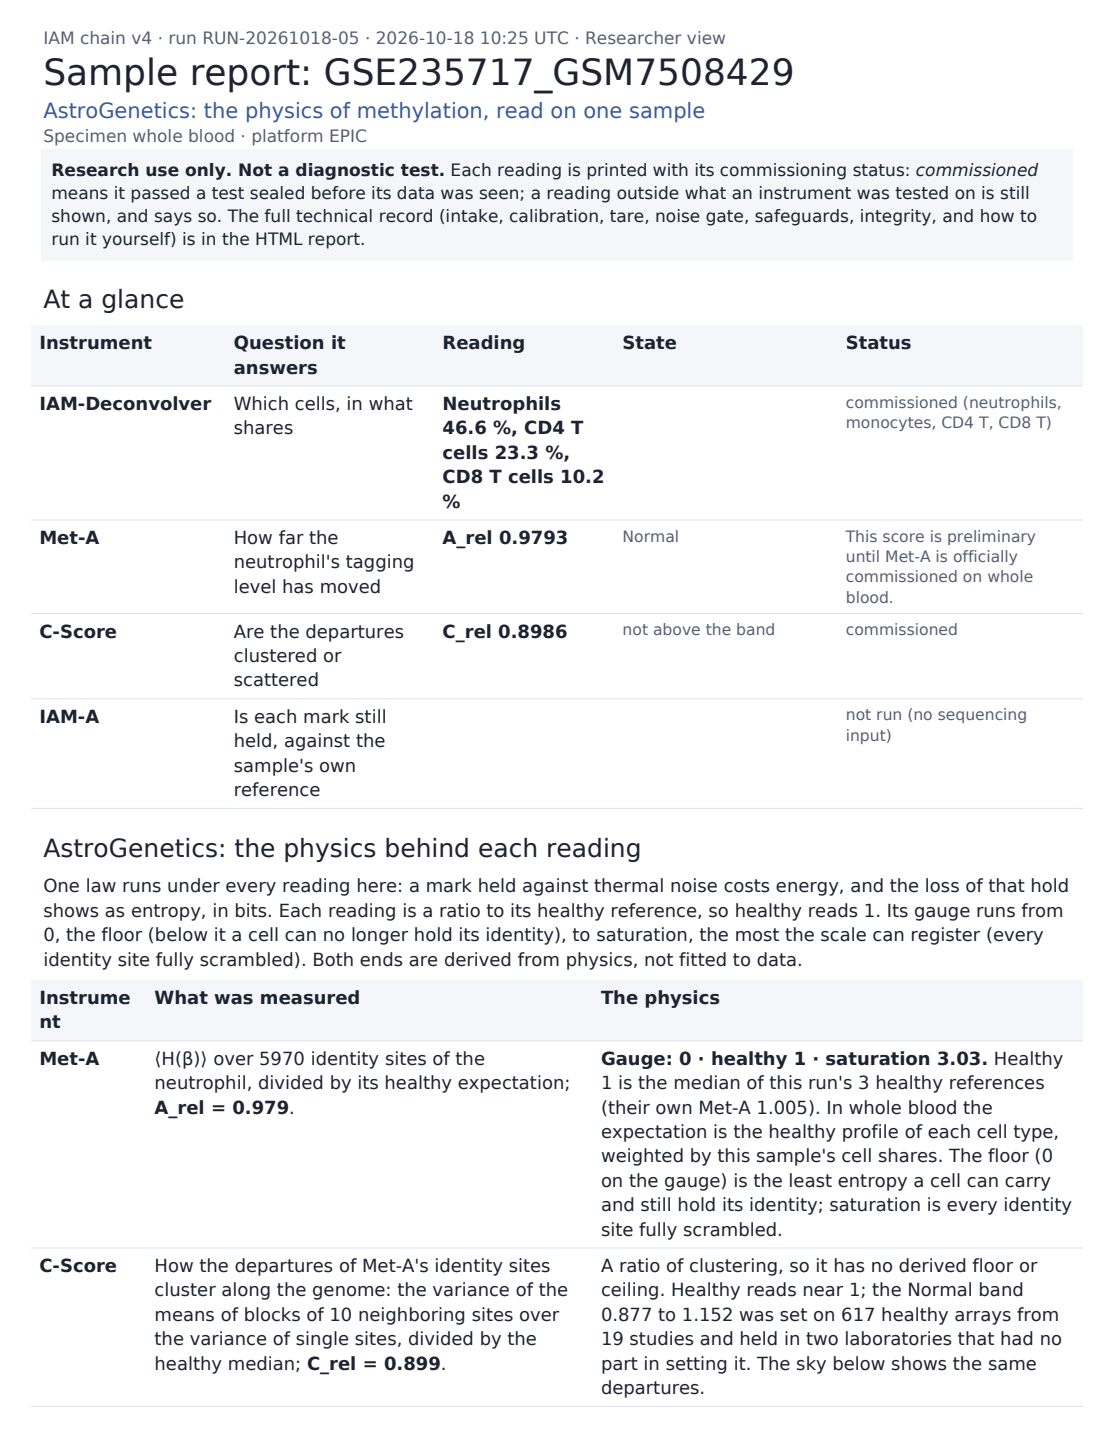
\includegraphics[width=0.92\textwidth,height=0.82\textheight,keepaspectratio]{figures/part6/fig_p6_report_blood_p1.png}
\caption{Healthy whole blood (GSE235717, GSM7508429), page 1: the reading of every instrument at a glance, each with its commissioning status (Met-A's whole-blood reading is labeled preliminary), and the physics behind each reading.}\label{fig:report:blood1}
\end{figure}

\begin{figure}[p]\centering
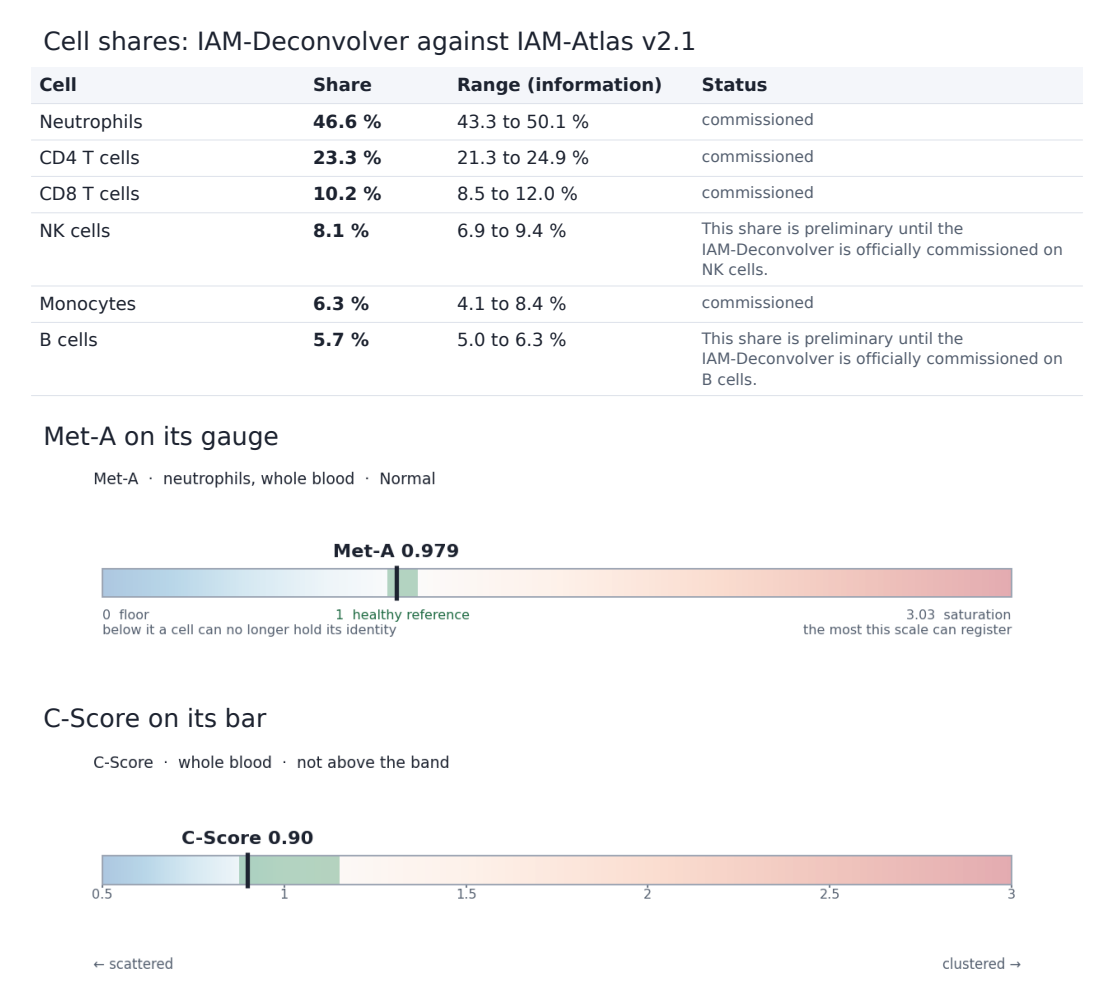
\includegraphics[width=0.92\textwidth,height=0.82\textheight,keepaspectratio]{figures/part6/fig_p6_report_blood_p2.png}
\caption{Page 2: the cell shares from the IAM-Deconvolver against IAM-Atlas v2.1, each with its range and status (NK and B cells are labeled preliminary), then Met-A on its gauge and the C-Score on its bar.}\label{fig:report:blood2}
\end{figure}

\begin{figure}[p]\centering
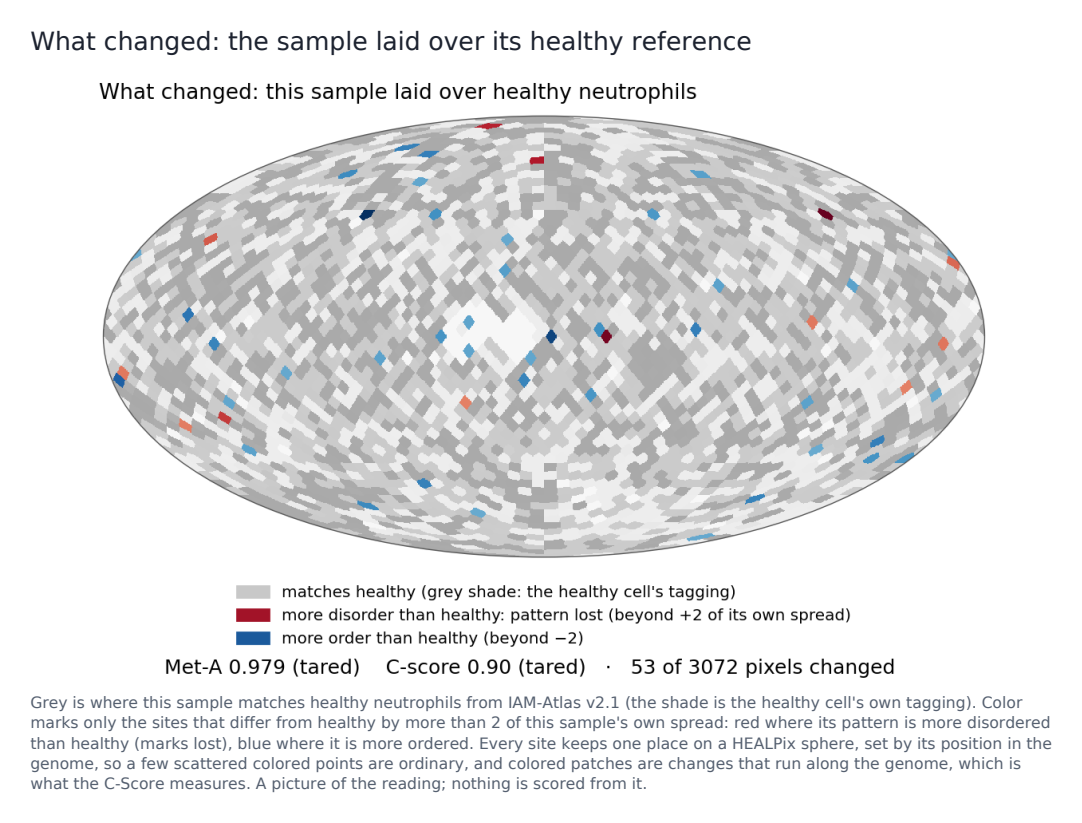
\includegraphics[width=0.92\textwidth,height=0.82\textheight,keepaspectratio]{figures/part6/fig_p6_report_blood_p3.png}
\caption{Page 3: what changed, the sample laid over its healthy reference on the HEALPix sphere. Gray is where the sample matches healthy neutrophils from IAM-Atlas v2.1; color marks only the sites that differ from healthy by more than 2 of the sample's own spread.}\label{fig:report:blood3}
\end{figure}

\begin{figure}[p]\centering
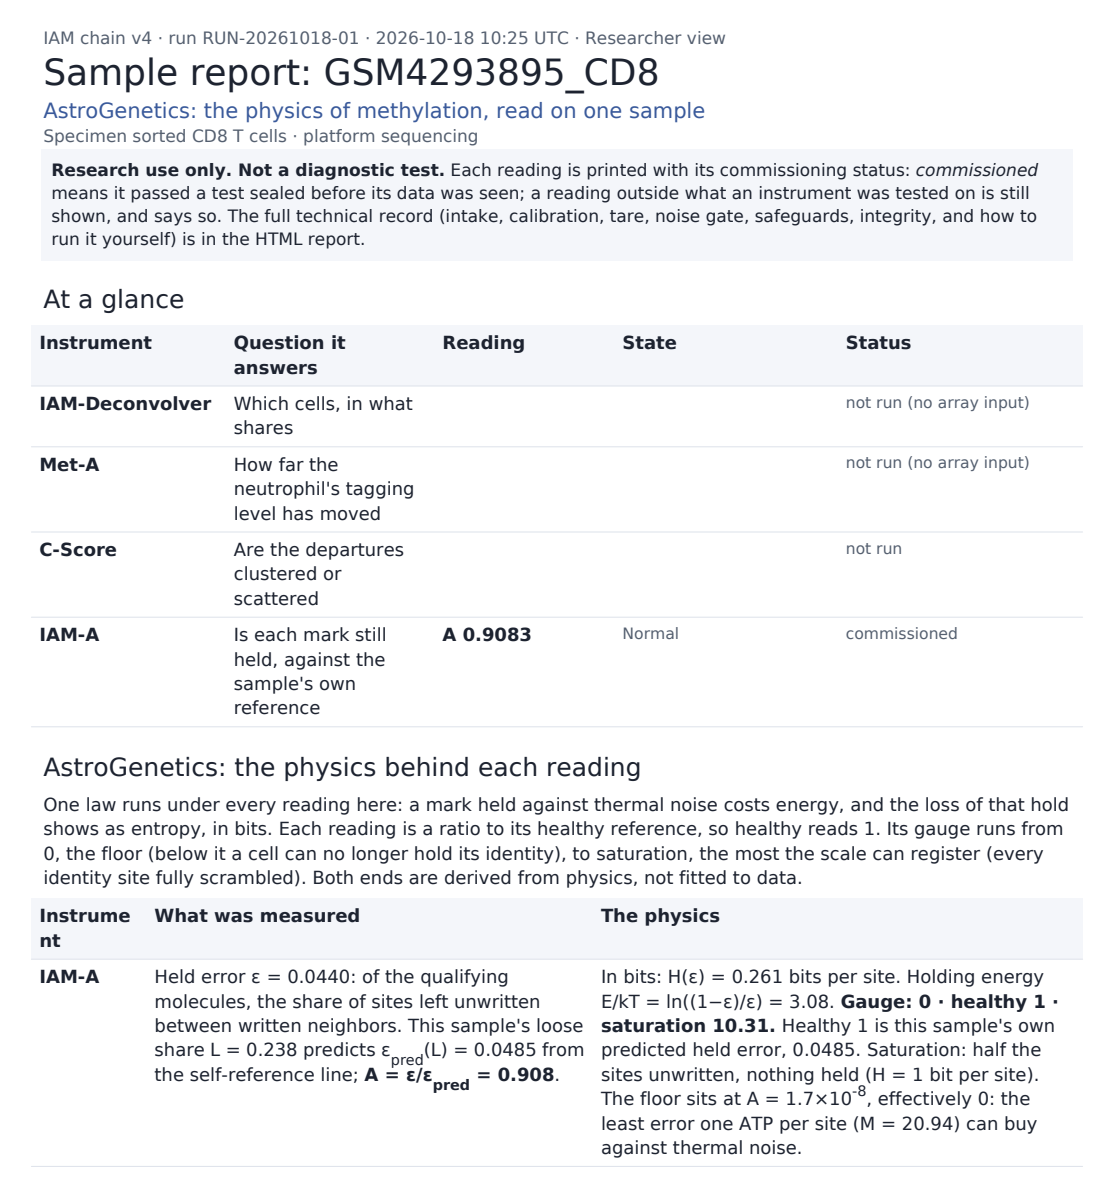
\includegraphics[width=0.92\textwidth,height=0.82\textheight,keepaspectratio]{figures/part6/fig_p6_report_cd8_p1.png}
\caption{Healthy CD8 T cells by sequencing (GSM4293895), page 1: IAM-A read against the sample's own reference (A 0.9083, Normal, commissioned): the held error, the loose share and what the healthy line predicts from it.}\label{fig:report:cd81}
\end{figure}

\begin{figure}[p]\centering
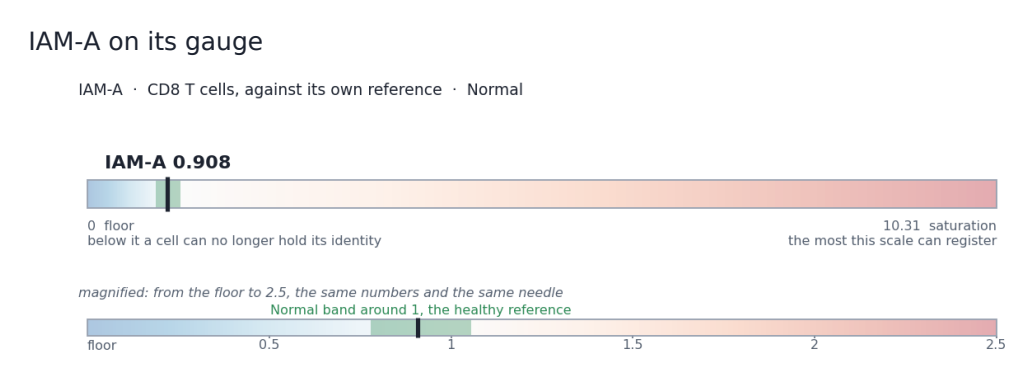
\includegraphics[width=0.92\textwidth,height=0.82\textheight,keepaspectratio]{figures/part6/fig_p6_report_cd8_p2.png}
\caption{Page 2: IAM-A on its gauge.}\label{fig:report:cd82}
\end{figure}

\clearpage
\section{Every result, rebuilt from public data}

Each test below is one entry in the repository's reproduction registry (Biological_Physics/MethylPhys/reproduce/tests.json). The command \texttt{python3 Biological_Physics/MethylPhys/reproduce/reproduce.py <test>} downloads only public files (GEO, ArrayExpress, ENCODE, the NCI Genomic Data Commons, ENA, Zenodo), runs the steps, and compares every number with the committed result, taken from git so a script cannot compare a file with itself. Each was run from a fresh clone of the public repository on a new machine.
 8 of the 9 tests have passed that way with every compared number identical.

\begin{center}\small\begin{tabular}{p{0.34\textwidth}p{0.22\textwidth}p{0.12\textwidth}p{0.18\textwidth}}\hline
\textbf{Test} & \textbf{Instrument} & \textbf{Checks} & \textbf{Fresh-clone result}\\\hline
\texttt{metaa\_rebuild} & Met-A (commissioned) & 8 of 8 & PASS, 2026-10-18\\
\texttt{deconv} & IAM-Deconvolver (commissioned) & 5 of 5 & PASS, 2026-10-18\\
\texttt{cscore\_band} & C-Score (commissioned) & 7 of 7 & PASS, 2026-10-18\\
\texttt{iama\_line} & IAM-A (commissioned) & 3 of 3 & PASS, 2026-10-18\\
\texttt{three\_labs} & Met-A and C-Score & 4 of 4 & PASS, 2026-10-18\\
\texttt{mice} & IAM-A (physics prediction) & -- & not yet recorded\\
\texttt{colon} & Met-A on tissue, with IAM-Atlas v2 & 6 of 6 & PASS, 2026-10-18\\
\texttt{breast} & Met-A on tissue, with IAM-Atlas v2 & 6 of 6 & PASS, 2026-10-18\\
\texttt{liver} & Met-A on tissue, with IAM-Atlas v2 & 6 of 6 & PASS, 2026-10-18\\
\hline\end{tabular}\end{center}

\subsection*{Met-A's reference, rebuilt from public arrays: noise sites and gate, the floor, the 6,000 identity sites, the healthy spread and the blood-composition markers}

Every reference matrix Met-A reads is rebuilt from 91 public purified-blood arrays and comes out identical to the frozen file the chain reads.

\begin{itemize}\setlength\itemsep{1pt}
\item \textbf{Public data:} GSE110554; GSE167998; GSE2998xxx neutrophil arrays (listed in reference\_donors.csv).
\item \textbf{Command:} \texttt{python3 Biological_Physics/MethylPhys/reproduce/reproduce.py metaa\_rebuild} (about 3 h; 20 GB of disk).
\item \textbf{Fresh-clone result:} PASS on 2026-10-18, 8 of 8 compared numbers identical, 110 minutes, repository commit \texttt{79a267d2}.
\item \textbf{Record:} \url{https://github.com/hmahaffeyges/IAM-Validation/blob/main/Biological_Physics/MethylPhys/doors/COMMISSIONING_NOTE_METAA_NEUTROPHILS.md}
\end{itemize}

\subsection*{Blood-cell shares in 200 mixtures from a laboratory the atlas never saw (E-MTAB-2145)}

The Deconvolver reads 200 mixtures of purified cells from an unseen laboratory within 0.016 of the true shares, and its sample check refuses the arrays that do not read as their own cell.

\begin{itemize}\setlength\itemsep{1pt}
\item \textbf{Public data:} E-MTAB-2145 (ArrayExpress).
\item \textbf{Command:} \texttt{python3 Biological_Physics/MethylPhys/reproduce/reproduce.py deconv} (about 30 min; 2 GB of disk).
\item \textbf{Fresh-clone result:} PASS on 2026-10-18, 5 of 5 compared numbers identical, 67 minutes, repository commit \texttt{537984a4}.
\item \textbf{Record:} \url{https://github.com/hmahaffeyges/IAM-Validation/blob/main/Biological_Physics/MethylPhys/doors/COMMISSIONING_NOTE_DECONV_V21.md}
\end{itemize}

\subsection*{The C-Score's healthy range holds in a laboratory that did not set it (GSE184269)}

Healthy whole bloods from a second laboratory read inside the C-Score band: 22 of 23 not above 1.152, the bar sealed before the arrays were fetched.

\begin{itemize}\setlength\itemsep{1pt}
\item \textbf{Public data:} GSE184269.
\item \textbf{Command:} \texttt{python3 Biological_Physics/MethylPhys/reproduce/reproduce.py cscore\_band} (about 40 min; 3 GB of disk).
\item \textbf{Fresh-clone result:} PASS on 2026-10-18, 7 of 7 compared numbers identical, 42 minutes, repository commit \texttt{537984a4}.
\item \textbf{Record:} \url{https://github.com/hmahaffeyges/IAM-Validation/blob/main/Biological_Physics/MethylPhys/doors/CSCORE_COMMISSIONING_PLAN.md}
\end{itemize}

\subsection*{IAM-A's self-reference line, rebuilt from 158 public healthy-cell sequencing files}

Every healthy cell type's held error falls on one simple line; recounted from GEO and ENCODE files through chain Stage Q2, every count, the line and the sample-shape reference come out identical.

\begin{itemize}\setlength\itemsep{1pt}
\item \textbf{Public data:} GSE186458 (153 .pat files, GEO); ENCODE ENCFF092SBB, ENCFF605NRU, ENCFF133QNK, ENCFF704SCQ, ENCFF969NGH; ENCODE GRCh38 analysis set.
\item \textbf{Command:} \texttt{python3 Biological_Physics/MethylPhys/reproduce/reproduce.py iama\_line} (about 3 h on 16 cores; 70 GB of disk; 32 GB of memory).
\item \textbf{Fresh-clone result:} PASS on 2026-10-18, 3 of 3 compared numbers identical, 168 minutes, repository commit \texttt{d27b4956}.
\item \textbf{Record:} \url{https://github.com/hmahaffeyges/IAM-Validation/blob/main/Biological_Physics/MethylPhys/doors/COMMISSIONING_NOTE_IAMA.md}
\end{itemize}

\subsection*{The same DNA gives the same reading in three laboratories (SEQC2 EpiQC, GSE230132)}

Identical cell-line DNA run at three laboratories: Met-A's technical repeats agree within 0.0114 and the same DNA across laboratories within 0.0084.

\begin{itemize}\setlength\itemsep{1pt}
\item \textbf{Public data:} GSE230132.
\item \textbf{Command:} \texttt{python3 Biological_Physics/MethylPhys/reproduce/reproduce.py three\_labs} (about 30 min; 3 GB of disk).
\item \textbf{Fresh-clone result:} PASS on 2026-10-18, 4 of 4 compared numbers identical, 36 minutes, repository commit \texttt{0654f813}.
\item \textbf{Record:} \url{https://github.com/hmahaffeyges/IAM-Validation/blob/main/Biological_Physics/MethylPhys/doors/DEV_EPIQC_ARRAY_01_OUTCOME.md}
\end{itemize}

\subsection*{Physics called it in advance, in living mice (GSE77079)}

Mice that cannot make enough of the methyl donor hold their marks worse, by the amount the law predicted before the data were read: knockout over wild type 1.124, inside the sealed window 1.016 to 1.135 (p 0.0003).

\begin{itemize}\setlength\itemsep{1pt}
\item \textbf{Public data:} GSE77079 (38 RRBS runs, ENA); UCSC mm10.
\item \textbf{Command:} \texttt{python3 Biological_Physics/MethylPhys/reproduce/reproduce.py mice} (about 10 h on 16 cores (mm10 index 100 min, then 38 runs at about 12 min each); 40 GB of disk; 64 GB (bwa mem on the converted mm10 index with 16 threads is killed at 32 GB) of memory).
\item \textbf{Fresh-clone result:} not yet recorded.
\item \textbf{Record:} \url{https://github.com/hmahaffeyges/IAM-Validation/blob/main/Biological_Physics/MethylPhys/doors/DEV_SAM_LEVER_01_OUTCOME.md}
\end{itemize}

\subsection*{Colorectal tumors leave their own healthy tissue's range (GSE131013, 88 patients)}

Each tumor read against the same patient's adjacent normal tissue at the atlas's composition-blind sites: 28 of 88 pairs above the bar fixed on normal pairs alone (11 needed), the sealed fingerprint verdict.

\begin{itemize}\setlength\itemsep{1pt}
\item \textbf{Public data:} GSE131013 (GEO); IAM-Atlas v2, Zenodo 10.5281/zenodo.23325865.
\item \textbf{Command:} \texttt{python3 Biological_Physics/MethylPhys/reproduce/reproduce.py colon} (about 2 h; 15 GB of disk).
\item \textbf{Fresh-clone result:} PASS on 2026-10-18, 6 of 6 compared numbers identical, 189 minutes, repository commit \texttt{0a4dc7aa}.
\item \textbf{Record:} \url{https://github.com/hmahaffeyges/IAM-Validation/blob/main/Biological_Physics/MethylPhys/doors/DEV_TISSUE_COLON_01_OUTCOME.md}
\end{itemize}

\subsection*{Breast cancer: tumors leave the patient's own healthy range far more often than chance}

Each tumor read against the same patient's healthy tissue at the atlas's composition-blind sites: 23 of 53 pairs above the bar fixed on normal pairs alone (about 3 expected by chance), the sealed fingerprint verdict.

\begin{itemize}\setlength\itemsep{1pt}
\item \textbf{Public data:} TCGA-BRCA 450K (NCI GDC open access); IAM-Atlas v2, Zenodo 10.5281/zenodo.23325865.
\item \textbf{Command:} \texttt{python3 Biological_Physics/MethylPhys/reproduce/reproduce.py breast} (about 2 h; 20 GB of disk).
\item \textbf{Fresh-clone result:} PASS on 2026-10-18, 6 of 6 compared numbers identical, 113 minutes, repository commit \texttt{211e26c0}.
\item \textbf{Record:} \url{https://github.com/hmahaffeyges/IAM-Validation/blob/main/Biological_Physics/MethylPhys/doors/DEV_TISSUE_BREAST_01_OUTCOME.md}
\end{itemize}

\subsection*{Liver cancer: a third cancer, the same result}

Each tumor read against the same patient's healthy tissue at the atlas's composition-blind sites: 22 of 50 pairs above the bar fixed on normal pairs alone (about 2 expected by chance), the sealed fingerprint verdict.

\begin{itemize}\setlength\itemsep{1pt}
\item \textbf{Public data:} TCGA-LIHC 450K (NCI GDC open access); IAM-Atlas v2, Zenodo 10.5281/zenodo.23325865.
\item \textbf{Command:} \texttt{python3 Biological_Physics/MethylPhys/reproduce/reproduce.py liver} (about 2 h; 20 GB of disk).
\item \textbf{Fresh-clone result:} PASS on 2026-10-18, 6 of 6 compared numbers identical, 139 minutes, repository commit \texttt{211e26c0}.
\item \textbf{Record:} \url{https://github.com/hmahaffeyges/IAM-Validation/blob/main/Biological_Physics/MethylPhys/doors/DEV_TISSUE_LIVER_01_OUTCOME.md}
\end{itemize}

